
\documentclass[reqno,11pt]{amsart}

%\usepackage{color,graphicx}
%\usepackage{mathrsfs,amsbsy}
\usepackage{amssymb}
\usepackage{amsmath}
\usepackage{amsfonts}
\usepackage{booktabs}
\usepackage{bm}
\usepackage{graphicx}
\usepackage{amsthm}
\usepackage{physics}
\usepackage{enumerate}
\usepackage[mathscr]{eucal}
\usepackage{float}
\usepackage{mathrsfs}
\usepackage{multicol}
\usepackage{multirow}
\usepackage[all,pdf]{xy}
\usepackage[a4paper,left=3cm,right=3cm]{geometry}
\usepackage[table,xcdraw]{xcolor} % before tikz-cd
\usepackage{tikz-cd}
\usepackage{hyperref}
\hypersetup{
colorlinks=true,
linkcolor=blue,
urlcolor=blue,
}
\usepackage{quiver} 
\usepackage{changepage}
\usepackage{extpfeil} %for longer arrows
%\usepackage[notcite,notref]{showkeys}
\usepackage{tikz}
\usetikzlibrary {backgrounds,calc,intersections,through}
\usetikzlibrary {positioning,shapes.misc}
% showkeys  make label explicit on the paper


\definecolor{ashgrey}{rgb}{0.7, 0.75, 0.71}
\makeatletter
\@namedef{subjclassname@2010}{%
  \textup{2010} Mathematics Subject Classification}
\makeatother

\numberwithin{equation}{section}

\theoremstyle{plain}
\newtheorem{theorem}{Theorem}[section]
\newtheorem{lemma}[theorem]{Lemma}
\newtheorem{proposition}[theorem]{Proposition}
\newtheorem{corollary}[theorem]{Corollary}
\newtheorem{claim}[theorem]{Claim}
\newtheorem{defn}[theorem]{Definition}
\newtheorem{ques}[theorem]{Question}
\newtheorem*{fact}{Facts}
\newtheorem{eg}[theorem]{Example}

\theoremstyle{plain}
\newtheorem{thmsub}{Theorem}[subsection]
\newtheorem{lemmasub}[thmsub]{Lemma}
\newtheorem{corollarysub}[thmsub]{Corollary}
\newtheorem{propositionsub}[thmsub]{Proposition}
\newtheorem{defnsub}[thmsub]{Definition}

\numberwithin{equation}{section}


\theoremstyle{remark}

\newtheorem{remark}[theorem]{Remark}
\newtheorem{remarks}{Remarks}
\newtheorem*{remarkstar}{Remark}
\newtheorem*{problem}{Question}
\newtheorem*{answer}{Answer}
\newtheorem*{easyex}{Easy exercise}
%\renewcommand\thefootnote{\fnsymbol{footnote}}
%dont use number as footnote symbol, use this command to change
\DeclareMathOperator{\chara}{\operatorname{char}}
\DeclareMathOperator{\supp}{supp}
\DeclareMathOperator{\dist}{dist}
\DeclareMathOperator{\vol}{vol}
\DeclareMathOperator{\diag}{diag}
%\DeclareMathOperator{\tr}{tr}
\DeclareMathOperator{\Img}{\operatorname{Im}}
\DeclareMathOperator{\Id}{\operatorname{Id}}
\DeclareMathOperator{\Rep}{\operatorname{Rep}}
\DeclareMathOperator{\Mod}{\operatorname{Mod}}
\DeclareMathOperator{\Hom}{\operatorname{Hom}}
\DeclareMathOperator{\Ext}{\operatorname{Ext}}
\DeclareMathOperator{\gldim}{\operatorname{gl.dim}}
\DeclareMathOperator{\projdim}{\operatorname{proj.dim}}
\DeclareMathOperator{\injdim}{\operatorname{inj.dim}}
\DeclareMathOperator{\dimv}{\operatorname{\underline{\mathbf{dim}}}}
\DeclareMathOperator{\SL}{\operatorname{SL}}
\DeclareMathOperator{\PGL}{\operatorname{PGL}}
\DeclareMathOperator{\Flagd}{\operatorname{Flag}_{d}}
\DeclareMathOperator{\Flagdstr}{\operatorname{Flag}_{d,str}}
\newcommand{\Gr}{\operatorname{Gr}}
\newcommand{\Grr}{\operatorname{Gr}}
\newcommand{\Grq}{\operatorname{Gr}^{KQ}}
\newcommand{\Flag}[1]{\operatorname{Flag}_{#1}}
\newcommand{\Flagstr}[1]{\operatorname{Flag}_{#1,str}}
\newcommand{\dimvec}[1]{#1}
\newcommand{\rderiv}[2]{\mathrm{R}^{#1}\! {#2}}
\newcommand{\ord}{\operatorname{ord}}
\newcommand{\orde}{\operatorname{ord}_e }
\newcommand{\representation}[2]{\genfrac{}{}{0pt}{3}{\phantom{000}#2\phantom{00}}{#1}}
\newcommand{\Spec}{\operatorname{Spec}}
\newcommand{\Proj}{\operatorname{Proj}}
\newcommand{\Pic}{\operatorname{Pic}}
\newcommand{\Coh}{\operatorname{Coh}}
\newcommand{\Psh}{\operatorname{Psh}}
\newcommand{\Sch}{\operatorname{Sch}}
\newcommand{\Schk}{\operatorname{Sch}_{k}}
\newcommand{\SchX}{\operatorname{Sch}_{X}}
\newcommand{\Set}{\operatorname{Set}}
\newcommand{\Ob}{\operatorname{Ob}}
\newcommand{\Mor}{\operatorname{Mor}}
\newcommand{\Hilb}{\operatorname{Hilb}}
\newcommand{\Quot}{\operatorname{Quot}}
\newcommand{\Sym}{\operatorname{Sym}}
\setlength\intextsep{0cm}
\setlength\textfloatsep{0cm}


\makeatletter
\newcommand\subsectiondisappear{\@startsection{subsubsection}{2}%
  \z@{.5\linespacing\@plus.7\linespacing}{-.5em}%
  {\normalfont\bfseries}}
\makeatother

\makeatletter
%Table of Contents
\setcounter{tocdepth}{3}

% Add bold to \section titles in ToC and remove . after numbers
\renewcommand{\tocsection}[3]{%
  \indentlabel{\@ifnotempty{#2}{\bfseries\ignorespaces#1 #2\quad}}\bfseries#3}
% Remove . after numbers in \subsection
\renewcommand{\tocsubsection}[3]{%
  \indentlabel{\@ifnotempty{#2}{\ignorespaces#1 #2\quad}}#3}
%\let\tocsubsubsection\tocsubsection% Update for \subsubsection
%...

\newcommand\@dotsep{4.5}
\def\@tocline#1#2#3#4#5#6#7{\relax
  \ifnum #1>\c@tocdepth % then omit
  \else
    \par \addpenalty\@secpenalty\addvspace{#2}%
    \begingroup \hyphenpenalty\@M
    \@ifempty{#4}{%
      \@tempdima\csname r@tocindent\number#1\endcsname\relax
    }{%
      \@tempdima#4\relax
    }%
    \parindent\z@ \leftskip#3\relax \advance\leftskip\@tempdima\relax
    \rightskip\@pnumwidth plus1em \parfillskip-\@pnumwidth
    #5\leavevmode\hskip-\@tempdima{#6}\nobreak
    \leaders\hbox{$\m@th\mkern \@dotsep mu\hbox{.}\mkern \@dotsep mu$}\hfill
    \nobreak
    \hbox to\@pnumwidth{\@tocpagenum{\ifnum#1=1\bfseries\fi#7}}\par% <-- \bfseries for \section page
    \nobreak
    \endgroup
  \fi}
\AtBeginDocument{%
\expandafter\renewcommand\csname r@tocindent0\endcsname{0pt}
}
\def\l@subsection{\@tocline{2}{0pt}{2.5pc}{5pc}{}}
\makeatother
%Table of contents in amsart: https://tex.stackexchange.com/questions/322268/table-of-contents-amsart
\begin{document}
\date{}

\title
{Moduli in Algebraic Geometry}


\author{Xiaoxiang Zhou}
\address{School of Mathematical Sciences\\
University of Bonn\\
Bonn, 53115\\ Germany\\} 
\email{email:xx352229@mail.ustc.edu.cn}





\begin{abstract}
In this personal survey, we conclude the definitions of moduli functors in the algebraic geometry. Most of the results are in the black box, so it's very possible that they're wrong. And also I'm not responsible for the completeness of the whole theory. I make no claim to originality. However, I'm still happy to improve this document, and make it better over time.

\end{abstract}

\setcounter{tocdepth}{2}
\maketitle
\tableofcontents 
%%%%%%%%%%%%%%%%%%%%%%%%%%%%%%%%%%%%%%%%%%%%%%%%%%%%%%%%%%%%%%%%%%%%%%%%%%%%%%%%%%%%%%%%%%%%%
\section{Goal and related concepts}
The personal survey is motivated by the three courses in Bonn: \href{https://johannesschmitt.gitlab.io/moduli_of_curves}{``the moduli space of curves"}, \href{https://www.math.uni-bonn.de/people/mihatsch/21u22\%20WS/moduli/}{``moduli of elliptic curves"} and \href{https://www.math.uni-bonn.de/people/ydutta/v5a4}{``moduli of vector bundles"}. I would also highly recommend the course \href{https://userpage.fu-berlin.de/hoskins/moduli_and_GIT.html}{``Moduli and GIT"} in Freie Universität Berlin. This is also partially covered by Dinamo Djounvouna's \href{https://www.math.u-bordeaux.fr/~ybilu/algant/documents/theses/Djounvouna.pdf}{master thesis}.  I want to construct my personal understanding on the moduli, and find out the details I missed in the courses. 

``Some mathematicians are birds, others
are frogs." This document is devoted to those ``birds" from a ``frog" who gets stuck in the mud.
\subsection{Conventions and Notations}
In this survey,  $\Schk$ is denoted as the category of \textbf{locally Noetherian} schemes over $k$, where $k$ is a field or $\mathbb{Z}$ or $\mathbb{Z}\left[\textstyle\frac{1}{6}\right]$.
\subsection{Representable functor}
In this subsection we would follow on \cite[Definition 2.2.1]{huybrechts2010geometry} in full generality, but you can always think 
$$\mathcal{C}=\Schk \qquad \mathcal{C}'=\operatorname{Functor} (\Schk^{op},\Set)$$
to visualize the statement, and you can refer to \cite[6.6.2]{FOAG} to see basic examples.
\begin{defn}[Functor category]
Fix a category $\mathcal{C}$, we define the corresponding functor category $\mathcal{C}'$ as follows:
% https://q.uiver.app/?q=WzAsMixbMCwwLCJcXG1hdGhjYWx7Q31ee29wfSJdLFsxLDAsIlxcU2V0Il0sWzAsMSwiIiwwLHsiY3VydmUiOjF9XSxbMCwxLCIiLDIseyJjdXJ2ZSI6LTF9XSxbMywyLCIiLDIseyJzaG9ydGVuIjp7InNvdXJjZSI6MjAsInRhcmdldCI6MjB9fV1d
$$\Ob(\mathcal{C}'):=\left\{  \text{functors }\mathcal{C}^{op}\longrightarrow \Set \right\} \qquad \Mor(\mathcal{C}'):=\left\{ \text{natural trans }
\begin{tikzcd}
	{\mathcal{C}^{op}} & \Set
	\arrow[""{name=0, anchor=center, inner sep=0}, curve={height=9pt}, from=1-1, to=1-2]
	\arrow[""{name=1, anchor=center, inner sep=0}, curve={height=-9pt}, from=1-1, to=1-2]
	\arrow[shorten <=2pt, shorten >=2pt, Rightarrow, from=1, to=0]
\end{tikzcd}
\right\}$$
In brief, $\mathcal{C}'=\operatorname{Functor} (\mathcal{C}^{op},\Set)$.\footnote{From  \href{https://userpage.fu-berlin.de/hoskins/moduli_and_GIT.html}{here} we can also write $\mathcal{C}'=\Psh(C)$, notice that here it is the presheaf on \textbf{category}, not on a specific scheme $X/k$.}
\end{defn}
\begin{proposition}
We have a canonical functor 
$$\iota: \mathcal{C} \longrightarrow \mathcal{C}' \qquad X \longmapsto h_X:=\Mor_{\mathcal{C}}(-,X)$$ which embeds $\mathcal{C}$ as a full subcategory of $\mathcal{C}'$.\footnote{$h_X$ is called the functor of points of a scheme $X$ from  \href{https://userpage.fu-berlin.de/hoskins/moduli_and_GIT.html}{here}. For example, $h_X(\Spec \mathbb{Q})=X(\mathbb{Q})$ gives us the set of rational points in $X$(under certain conditions). Notice that $h_{-}(-)$ is a bifunctor.}
\end{proposition}
\begin{proof}
Recall that the Yoneda's lemma gives us the isomorphism
$$\Mor_{\mathcal{C}'}(h_X,F)\cong F(X).$$
\end{proof}
\begin{defn}[Representable functor]\label{def:repfctor}
The functor $F\in \Ob(\mathcal{C}')$ is called represented by $X$ if $F\cong h_X$.
\end{defn}
From this proposition, we can always view the object as some functor satisfying some properties. we get three advantages from this point of view:
\begin{itemize}
\item It's easy to see rational points and complex points;
\item We can define scheme canonically, without explicit constructions;
\item We can enlarge our area of research, and think them as the defective schemes. We will see some reasonable functors which is represented not by schemes, but by stacks.
\end{itemize}
\begin{remark}
By \cite[1.3.6]{vistoli2004notes}, any representable functor (after restricted to specific subcategory of $\mathcal{C}=\Schk$) is a sheaf in Zariski/étale/fppf/fpqc topology.
\end{remark}
\subsection{Corepresentable functor}
This is the concept "dual to" the representable functor. To motivate, we begin with the equivalent definition of representable functor:
\begin{defn}[Representatable functor, equivalent definition]
A functor $F\in \Ob(\mathcal{C}')$ is represented by $X \in \Ob(C)$ if $F$ satisfies the following universal properties:
\begin{itemize}
\item There exists a morphism $\eta^{-1}:h_X \longrightarrow F$ in $\Mor_{\mathcal{C}'}(h_X,F)$;
\item For any object $X' \in \Ob(\mathcal{C})$ and morphism $\alpha':h_{X'}\longrightarrow F$ in $\Mor_{\mathcal{C}'}(h_{X'},F)$, there exists an unique morphism $\beta \in \Mor_{\mathcal{C}}(X',X)$ such that $\alpha'=\eta^{-1} \circ h_{\beta}$.
% https://q.uiver.app/?q=WzAsNSxbMCwwXSxbMSwwLCJoX3tYJ30iXSxbMSwxLCJoX3tYfSJdLFsyLDBdLFsyLDEsIkYiXSxbMSwyLCJcXGV4aXN0IFxcLCEgXFwsaF97XFxiZXRhfSIsMix7ImNvbG91ciI6WzM1OCwxMDAsNTBdLCJzdHlsZSI6eyJib2R5Ijp7Im5hbWUiOiJkYXNoZWQifX19LFszNTgsMTAwLDUwLDFdXSxbMiw0LCJcXGFscGhhIiwyXSxbMSw0LCJcXGFscGhhJyJdXQ==
$$\begin{tikzcd}
	{} & {h_{X'}} & {} \\
	& {h_{X}} & F
	\arrow["{\exists \,! \,h_{\beta}}"', color={rgb,255:red,255;green,0;blue,8}, dashed, from=1-2, to=2-2]
	\arrow["\eta^{-1}"', from=2-2, to=2-3]
	\arrow["{\alpha'}", from=1-2, to=2-3]
\end{tikzcd}$$
\end{itemize}
\end{defn}
This definition is equivalent to the Definition \ref{def:repfctor} since \footnote{The middle isomorphism comes from the universal property, while the two equalities come from the Yoneda's lemma.}
$$h_X(X')=\Mor_{\mathcal{C}}(X',X) \cong \Mor_{\mathcal{C}'}(h_{X'},F) =F(X') \text{ for any } X'\in \Ob(\mathcal{C})$$
thus the functor $\eta^{-1}: h_X \longrightarrow F$ is an isomorphism.
\begin{defn}[Corepresentable functor]
A functor $F\in \Ob(\mathcal{C}')$ is corepresented by $X \in \Ob(C)$ if $F$ satisfies the following universal properties:
\begin{itemize}
\item There exists a morphism $\eta:F \longrightarrow h_X$ in $\Mor_{\mathcal{C}'}(F,h_X)$;
\item For any object $X' \in \Ob(\mathcal{C})$ and morphism $\alpha':F\longrightarrow h_{X'}$ in $\Mor_{\mathcal{C}'}(F,h_{X'})$, there exists an unique morphism $\beta \in \Mor_{\mathcal{C}}(X,X')$ such that $\alpha'=h_{\beta} \circ \eta$.
% https://q.uiver.app/?q=WzAsMyxbMCwwLCJGIl0sWzEsMCwiaF9YIl0sWzEsMSwiaF97WCd9Il0sWzAsMSwiXFxhbHBoYSJdLFsxLDIsIlxcZXhpc3QgXFwsISBcXCxoX3tcXGJldGF9IiwwLHsiY29sb3VyIjpbMzU4LDEwMCw1MF0sInN0eWxlIjp7ImJvZHkiOnsibmFtZSI6ImRhc2hlZCJ9fX0sWzM1OCwxMDAsNTAsMV1dLFswLDIsIlxcYWxwaGEnIiwyXV0=
$$\begin{tikzcd}
	F & {h_X} \\
	& {h_{X'}}
	\arrow["\eta", from=1-1, to=1-2]
	\arrow["{\exists \,! \,h_{\beta}}", color={rgb,255:red,255;green,0;blue,8}, dashed, from=1-2, to=2-2]
	\arrow["{\alpha'}"', from=1-1, to=2-2]
\end{tikzcd}$$
\end{itemize}
\end{defn}
\begin{defn}[Universal corepresentable functor]
A functor $F\in \Ob(\mathcal{C}')$ is universal corepresented by $X \in \Ob(C)$ if for any morphism $\gamma :Y\longrightarrow X$, the functor $F \times_{h_X} h_Y$ is corepresented by $Y$.
% https://q.uiver.app/?q=WzAsNCxbMCwxLCJGIl0sWzEsMSwiaF9YIl0sWzEsMCwiaF9ZIl0sWzAsMCwiRiBcXHRpbWVzX3toX1h9IGhfWSJdLFswLDEsIlxcYWxwaGEiXSxbMiwxLCJoX3tcXGdhbW1hfSJdLFszLDJdLFszLDBdXQ==
\[\begin{tikzcd}
	{F \times_{h_X} h_Y} & {h_Y} \\
	F & {h_X}
	\arrow["\alpha", from=2-1, to=2-2]
	\arrow["{h_{\gamma}}", from=1-2, to=2-2]
	\arrow[from=1-1, to=1-2]
	\arrow[from=1-1, to=2-1]
\end{tikzcd}\]
\end{defn}
\begin{proposition}
Suppose a functor $F\in \Ob(\mathcal{C}')$ is corepresented by $X \in \Ob(C)$, then it is represented by $X$ if and only if $\eta:F \longrightarrow h_X$ is a $\mathcal{C}'$-isomorphism.
\end{proposition}
\subsection{Coarse moduli space}
You need to see the definition of the naive moduli problem, extended moduli problem, moduli functor, fine moduli space and corresponding universal family from  \href{https://userpage.fu-berlin.de/hoskins/moduli_and_GIT.html}{here}. I don't want to copy, and it's well-written.

The following example will check if you really understand these concepts.
\begin{eg}[$\mathcal{M}_{0,3}$ is represented by one point $\Spec k$]\label{eg:M03}\

\textbf{Naive moduli problem} $(\mathcal{A},\sim)$:
$$\mathcal{A}:=\left\{(p_1,p_2,p_3)  \;\middle|\; p_i \in \mathbb{P}_k^1(k) \text{ are distinct } \right\}$$
$$(p_1,p_2,p_3) \sim (q_1,q_2,q_3) \Longleftrightarrow \exists \, \gamma \in \PGL_2(k) \text{ s.t. } q_i=\gamma(p_i)$$

\textbf{Extended moduli problem} $(\mathcal{A}_S,\sim_S)$ + pullback: \textcolor{gray}{$(S \in \Ob(\Schk))$}
$$\mathcal{A}_S:=\left\{(X,\pi,\sigma_1,\sigma_2,\sigma_3)  \;\middle|\; \begin{aligned}
&\\[-5mm]
&X \in \Ob(\Schk)\\[-1mm]
&\pi:X \longrightarrow S \text{ proper flat and }\pi^{-1}(p)\cong\mathbb{P}_{\kappa(p)}^1 \\[-1mm]
&\sigma_i:S \longrightarrow X \text{ pairwise disjoint sections of }\pi
\end{aligned}
 \right\}$$
 
 $(X,\pi,\sigma_1,\sigma_2,\sigma_3) \sim_S (X',\pi',\sigma_1',\sigma_2',\sigma_3')$ if there exists an isomorphism $f:X \longrightarrow X'$ such that the following diagrams commute:
   % https://q.uiver.app/?q=WzAsNixbMCwwLCJYIl0sWzIsMCwiWCciXSxbMSwxLCJTIl0sWzMsMCwiWCJdLFs0LDEsIlMiXSxbNSwwLCJYJyJdLFszLDUsImYiXSxbNCw1LCJcXHNpZ21hX2knIiwyXSxbNCwzLCJcXHNpZ21hX2kiXSxbMCwyLCJcXHBpIiwyXSxbMSwyLCJcXHBpJyJdLFswLDEsImYiXV0=
   \[\begin{tikzcd}[column sep=3mm]
   	X && {X'} &[20mm] X && {X'} \\
   	& S &&& S
   	\arrow["f", from=1-4, to=1-6]
   	\arrow["{\sigma_i'}"', from=2-5, to=1-6]
   	\arrow["{\sigma_i}", from=2-5, to=1-4]
   	\arrow["\pi"', from=1-1, to=2-2]
   	\arrow["{\pi'}", from=1-3, to=2-2]
   	\arrow["f", from=1-1, to=1-3]
   \end{tikzcd}\]
   
   For a map $f:T \longrightarrow S$, the pullback $f^*$ is defined by
   $$f^*:\mathcal{A}_S \longrightarrow \mathcal{A}_T \qquad (X,\pi,\sigma_1,\sigma_2,\sigma_3) \longmapsto (X_T,\pi_T,\sigma_{1,T},\sigma_{2,T},\sigma_{3,T})$$
   where $X_T$, $\pi_T$ are defined as fiber product, and $\sigma_{i,T}$ are defined by the universal property of fiber product, as follows:
   % https://q.uiver.app/?q=WzAsOSxbMCwxLCJYX1QiXSxbMSwxLCJYIl0sWzAsMiwiVCJdLFsxLDIsIlMiXSxbMywxLCJYX1QiXSxbMywyLCJUIl0sWzQsMiwiUyJdLFs0LDEsIlgiXSxbMiwwLCJUIl0sWzAsMiwiXFxwaV9UIiwyXSxbMiwzLCJmIl0sWzEsMywiXFxwaSJdLFs0LDUsIlxccGlfVCIsMl0sWzUsNiwiZiJdLFs3LDYsIlxccGkiLDJdLFs0LDddLFs4LDcsIlxcc2lnbWFfaSBcXGNpcmMgZiIsMCx7ImN1cnZlIjotMn1dLFs4LDQsIlxcZXhpc3RzIFxcLCFcXCwgXFxzaWdtYV97aSxUfSAiLDAseyJsYWJlbF9wb3NpdGlvbiI6OTAsImNvbG91ciI6WzAsMTAwLDUwXSwic3R5bGUiOnsiYm9keSI6eyJuYW1lIjoiZGFzaGVkIn19fSxbMCwxMDAsNTAsMV1dLFs4LDUsIlxcSWRfVCIsMix7ImN1cnZlIjoyfV0sWzYsNywiXFxzaWdtYV97aX0iLDIseyJjdXJ2ZSI6MSwic3R5bGUiOnsiYm9keSI6eyJuYW1lIjoiZGFzaGVkIn19fV0sWzAsMV0sWzAsMywiIiwxLHsic3R5bGUiOnsibmFtZSI6ImNvcm5lciJ9fV0sWzQsNiwiIiwxLHsic3R5bGUiOnsibmFtZSI6ImNvcm5lciJ9fV1d
   \[\begin{tikzcd}
   	&&[15mm] T&[-6mm] \\[-6mm]
   	{X_T} & X && {X_T} & X \\
   	T & S && T & S
   	\arrow["{\pi_T}"', from=2-1, to=3-1]
   	\arrow["f", from=3-1, to=3-2]
   	\arrow["\pi", from=2-2, to=3-2]
   	\arrow["{\pi_T}"', from=2-4, to=3-4]
   	\arrow["f", from=3-4, to=3-5]
   	\arrow["\pi"', from=2-5, to=3-5]
   	\arrow[from=2-4, to=2-5]
   	\arrow["{\sigma_i \circ f}", curve={height=-12pt}, from=1-3, to=2-5]
   	\arrow["{\exists \,!\, \sigma_{i,T} }"{pos=1.12}, color=red, dashed, from=1-3, to=2-4]
   	\arrow["{\Id_T}"', curve={height=12pt}, from=1-3, to=3-4]
   	\arrow["{\sigma_{i}}"', curve={height=6pt}, dashed, from=3-5, to=2-5]
   	\arrow[from=2-1, to=2-2]
   	\arrow["\ulcorner"{anchor=center, pos=0.125}, draw=none, from=2-1, to=3-2]
   	\arrow["\ulcorner"{anchor=center, pos=0.125}, draw=none, from=2-4, to=3-5]
   \end{tikzcd}\]
 \begin{adjustwidth}{10mm}{0em}
 \begin{remarkstar}
 We can always view the point $p \in S$ as an affine scheme of its residue field. So the two conditions below are equivalent:
 \begin{equation*}
 \begin{aligned}
  &\pi^{-1}(p)\cong\mathbb{P}_{\kappa(p)}^1& & \text{ for any } p \in S  \\ 
  &\pi^{-1}(\Spec L)\cong \mathbb{P}_{L}^1& & \text{ for any } \Spec L \hookrightarrow S  \\ 
 \end{aligned}
 \end{equation*}
 \end{remarkstar}
 \begin{remarkstar}
 In some textbooks, they require $\pi:X \longrightarrow S$ to be a smooth, proper, surjective, locally finitely presented (l.f.p.)
 morphism of relative dimension $\leqslant 1$ with geometric fibres isomorphic to $\mathbb{P}^1$. These extra conditions are automatically satisfied, since
 % https://q.uiver.app/?q=WzAsNixbMCwwLCJcXGJ1bGxldCJdLFsxLDAsIlxcdGV4dHtzdXJqZWN0aXZlfSJdLFsxLDEsIlxcYnVsbGV0Il0sWzAsMSwiXFxidWxsZXQiXSxbMSwyLCJcXGJ1bGxldCJdLFswLDIsIlxcYnVsbGV0Il0sWzAsMV0sWzAsMl0sWzMsMl0sWzMsNF0sWzUsNF1d
 \[\begin{tikzcd}[/tikz/column 1/.append style={anchor=base east},/tikz/column 2/.append style={anchor=base west}, column sep=3cm, row sep=-2mm,start anchor=east,end anchor=west]
 	\pi^{-1}(p)\cong\mathbb{P}_{\kappa(p)}^1 & {\text{surjective}} \\
 	{\text{proper}} & {\text{relative dimension $\leqslant 1$}} \\
 	{\text{locally Noetherian}} & {\text{locally finitely presented}}
 	\arrow[from=1-1, to=1-2]
 	\arrow[from=1-1, to=2-2]
 	\arrow[from=2-1, to=2-2]
 	\arrow[from=2-1, to=3-2]
 	\arrow[from=3-1, to=3-2]
 \end{tikzcd}\]
 and by \cite[25.2.2]{FOAG}, flat + fiberwise $\mathbb{P}^1$ + l.f.p. $\Rightarrow$ smooth. 
 
 \end{remarkstar}
\begin{problem}\hspace{1cm}

Can we find $(X,\pi,\sigma_1,\sigma_2,\sigma_3)$ satisfying all conditions in $\mathcal{A}_S$ except $\pi$ is separated? 

Can we find $(X,\pi,\sigma_1,\sigma_2,\sigma_3)$ satisfying all conditions in $\mathcal{A}_S$ except $\pi$ is flat?
\end{problem}
\begin{answer}
Still unknown. From Dr. Johannes Anschütz, the map
$$\mathbb{P}_k^1 \longrightarrow \Spec k \longrightarrow \Spec k[t]/t^2$$
is proper but not flat(sadly we can't find any section). If the base scheme $S$ is reduced, then maybe the flatness can be checked fiberwise?

Another obstruction for the flatness comes from \cite[26.2.11]{FOAG} or \href{https://math.stackexchange.com/questions/1704423/smooth-fibration-on-a-smooth-curve}{stackexchange}.
\end{answer}
\begin{easyex}\hspace{1cm}

Verify that $(\mathcal{A}_S,\sim_S)$ and pullback satisfy (i)-(iv) in \cite[Definition 2.10]{moduliGIT}.
\end{easyex}



 \end{adjustwidth}



\textbf{Moduli functor} $\mathcal{M}_{0,3}$:
The moduli functor $\mathcal{M}_{0,3}: \Schk^{op}\longrightarrow \Set$ is defined as
$$\mathcal{M}_{0,3}(S)=\mathcal{A}_S/\sim_S \qquad \mathcal{M}_{0,3}(f:T\longrightarrow S)=f^*: \mathcal{A}_S/\sim_S \longrightarrow \mathcal{A}_T/\sim_T.$$
\vspace{-1.1cm}
\begin{adjustwidth}{10mm}{0em}

\begin{problem}\hspace{1cm}

Why is the moduli functor $\mathcal{M}_{0,3}$ represented by $\Spec k$?
\end{problem}
\begin{answer}\hspace{1cm}

Yes, but it's pretty hard to prove it. The proof of \cite[Proposition 4.1]{modulicurve} uses \cite[Proposition 4.2]{modulicurve} whose proof is quite technical.

Actually we construct the natural functor $\eta^{-1}:h_{\Spec k} \longrightarrow \mathcal{M}_{0,3}$ by
$$\eta^{-1}_S:h_{\Spec k}(S) \longrightarrow \mathcal{M}_{0,3}(S) \qquad [S \rightarrow \Spec k] \longmapsto (\mathbb{P}_S^1=\mathbb{P}_k^1 \times_k S, pr_1,0,1,\infty)$$
and then verify that $\eta^{-1}_S$ is an isomorphism.
\end{answer}
\end{adjustwidth}
\textbf{Universal family}:
By \cite[Definition 2.16]{moduliGIT}, the universal family is $(\mathbb{P}_k^1, \pi,0,1,\infty)$.

\end{eg}

coarse moduli space and some related concepts. 
\subsection{Bigger category}
We need to define Grothendieck Topology and site, discussing how this generalized the language of scheme. Maybe I can follow \cite{moduliGIT}.

We need to define stack, algebraic stack, Deligne-Munford stack and some related concepts. Maybe I can follow \href{https://sites.math.washington.edu/~jarod/moduli.pdf}{Notes on Stacks and Moduli}. It seems like so nicely written.
\subsection{Goal}
???
\subsection{Quotient}
We will frequently use the quotient. Here is the list of quotients we've already seen:
\begin{itemize}
\item (We could begin at topology: quotient by a subset) linear space-> Abelian category,group,ring(Notice that for this item, we don't take quotient by a group, so sometimes it looks easier)
\item topology(This gives us an categorical quotient!)
\item manifold
\item scheme(Categorical quotient; GIT quotient)
\end{itemize}
See \cite{moduliGIT} for the following concepts:
\begin{itemize}
\item categorical quotients, good quotients, geometric quotients, and GIT quotients.
\item reductive, linearly reductive, and geometrically reductive.(see \cite[Theorem 4.16]{moduliGIT})
\item stable, semistable, unstable, and polystable.
\item Hilbert-Mumford Criterion and Fundamental Theorem in GIT.
\end{itemize}
See \cite{edixhoven2012abelian} for the following concepts:
\begin{itemize}
\item universal categorical quotients, universal geometric quotients.(4.5(iv), 4.12)
\item fppf quotient.(4.28)
\end{itemize}
% % https://q.uiver.app/?q=WzAsOSxbMCw0LCJcXHN1YnN0YWNre1xcdGV4dHtnZW9tZXRyaWMgcXVvdGllbnR9fSJdLFsxLDQsIlxcc3Vic3RhY2t7XFx0ZXh0e2dvb2QgcXVvdGllbnR9fSJdLFsyLDQsIlxcc3Vic3RhY2t7XFx0ZXh0e2NhdGVnb3JpY2FsIHF1b3RpZW50fX0iXSxbMSwzLCJcXHN1YnN0YWNre1xcdGV4dHtyZWR1Y3RpdmUgR0lUIHF1b3RpZW50fX0iXSxbMiwyLCJcXHN1YnN0YWNre1xcdGV4dHt1bml2ZXJzYWx9XFxcXCBcXHRleHR7Y2F0ZWdvcnVjYWwgcXVvdGllbnR9fSJdLFswLDIsIlxcc3Vic3RhY2t7XFx0ZXh0e3VuaXZlcnNhbH1cXFxcIFxcdGV4dHtnZW9tZXRyaWMgcXVvdGllbnR9fSJdLFswLDEsIlxcc3Vic3RhY2t7XFx0ZXh0e2ZwcGYgcXVvdGllbnR9fSJdLFsxLDEsIlxcc3Vic3RhY2t7XFx0ZXh0e2ZwcWMgcXVvdGllbnR9fSJdLFswLDAsIlxcc3Vic3RhY2t7XFx0ZXh0e8OpdGFsZSBxdW90aWVudH19Il0sWzAsMSwiIiwwLHsibGV2ZWwiOjJ9XSxbMSwyLCIiLDAseyJsZXZlbCI6Mn1dLFszLDEsIlxcc3Vic3RhY2t7XFx0ZXh0e1RobSA0LjMwfX0iLDAseyJsZXZlbCI6Mn1dLFszLDAsIlxcc3Vic3RhY2t7XFx0ZXh0e3N0YWJsZX19IiwwLHsic3R5bGUiOnsiYm9keSI6eyJuYW1lIjoiZGFzaGVkIn19fV0sWzUsNCwiIiwwLHsibGV2ZWwiOjJ9XSxbNSwwLCIiLDAseyJsZXZlbCI6Mn1dLFs0LDIsIiIsMSx7ImxldmVsIjoyfV0sWzYsNSwiIiwwLHsibGV2ZWwiOjJ9XSxbMCw2LCJcXHN1YnN0YWNre1xcdGV4dHthc3N1bXB0aW9uIGlufSBcXFxcIFxcdGV4dHtcXGNpdGVbKDQuMzUpKGlpKV17ZWRpeGhvdmVuMjAxMmFiZWxpYW59fX0iLDAseyJvZmZzZXQiOi01LCJjdXJ2ZSI6LTUsInN0eWxlIjp7ImJvZHkiOnsibmFtZSI6ImRhc2hlZCJ9fX1dLFs2LDcsIiIsMCx7ImxldmVsIjoyfV0sWzgsNiwiIiwwLHsibGV2ZWwiOjJ9XV0=
\[\begin{tikzcd}
	{\substack{\text{étale quotient}}} \\
	{\substack{\text{fppf quotient}}} & {\substack{\text{fpqc quotient}}} \\
	{\substack{\text{universal}\\ \text{geometric quotient}}} && {\substack{\text{universal}\\ \text{categorucal quotient}}} \\
	& {\substack{\text{reductive GIT quotient}}} \\
	{\substack{\text{geometric quotient}}} & {\substack{\text{good quotient}}} & {\substack{\text{categorical quotient}}}
	\arrow[Rightarrow, from=5-1, to=5-2]
	\arrow[Rightarrow, from=5-2, to=5-3]
	\arrow["{\substack{\text{Thm 4.30}}}", Rightarrow, from=4-2, to=5-2]
	\arrow["{\substack{\text{stable}}}", dashed, from=4-2, to=5-1]
	\arrow[Rightarrow, from=3-1, to=3-3]
	\arrow[Rightarrow, from=3-1, to=5-1]
	\arrow[Rightarrow, from=3-3, to=5-3]
	\arrow[Rightarrow, from=2-1, to=3-1]
	\arrow["{\substack{\text{assumption in} \\ \text{\cite[(4.35)(ii)]{edixhoven2012abelian}}}}", shift left=5, curve={height=-30pt}, dashed, from=5-1, to=2-1]
	\arrow[Rightarrow, from=2-1, to=2-2]
	\arrow[Rightarrow, from=1-1, to=2-1]
\end{tikzcd}\]
%%%%%%%%%%%%%%%%%%%%%%%%%%%%%%%%%%%%%%%%%%%%%%%%%%%%%%%%%%%%%%%%%%%%%%%%%%%%%%%%%%%%%%%%%%%%%
\section{Basic object}
In this section, we present some algebraic geometric objects which can be viewed as moduli.

Here is a picture showing the relationships of these objects:
% https://tikzcd.yichuanshen.de/#N4Igdg9gJgpgziAXAbVABwnAlgFyxMJZABgBpiBdUkANwEMAbAVxiRAB12BbOnACwBGA4AAUAvgDUQY0uky58hFGQCMVWoxZtOPfkNFidvPgGNGwAGJjpskBmx4CRFaTXV6zVog7sA4gCcACn9SCQBKGzkHRWdSACZ1Dy1vTgBFJggcSLt5RyUSeMTNLx8ACSwGAWz7BScUOML3Yu12CwY6AHMoQPDpdRgoDvgiUAAzfwguJDIQHAgkFRkxianEGbmkOKWQccnN6g3EAGZt3dWXWfnj05WkABYDq5PbM-3LpABWMQoxIA
\[\begin{tikzcd}[row sep={12mm,between origins}, column sep={15mm,between origins}]
\mathbb{P}V \arrow[d] \arrow[rd] &                                 &           \\
\mathbb{P}\mathcal{F} \arrow[rd] & {\Gr(r,V)} \arrow[d] \arrow[rd] &           \\
\Hilb \arrow[r]                  & \Quot                           & \Flagd(V)
\end{tikzcd}\]
\subsection{Projective space}
We begin with a basic extended moduli problem, and then gradually make some variations.
\begin{eg}[Moduli of line bundle with base-point-free sections is represented by $\mathbb{P}_k^n$]
Fix $n \geqslant 0$, we define a moduli problem:
$$\mathcal{A}_S:=\left\{(\mathcal{L},s_0,\ldots,s_n)  \;\middle|\; \begin{aligned}
&\\[-5mm]
&\mathcal{L} \in \Pic(S)\\[-1mm]
& s_i \in \Gamma(S,\mathcal{L}) \text{ with no common zero }
\end{aligned}
 \right\}$$
 
  $(\mathcal{L},s_0,\ldots,s_n) \sim_S (\mathcal{L}',s_0',\ldots,s_n')$ if there exists an isomorphism of line bundles $\phi:\mathcal{L} \longrightarrow \mathcal{L}'$ such that $\phi(S):\Gamma(S,\mathcal{L}) \longrightarrow \Gamma(S,\mathcal{L}')$ sends $s_i$ to $s_i'$.
  
  For a map $f:T \longrightarrow S$, the pullback $f^*$ is defined by
     $$f^*:\mathcal{A}_S \longrightarrow \mathcal{A}_T \qquad (\mathcal{L},s_0,\ldots,s_n) \longmapsto (f^*\mathcal{L},f^*s_0,\ldots,f^*s_n)$$
     
By \cite[15.3.F, 16.4.1]{FOAG}, the moduli functor defined by this extended moduli problem is represented by $\mathbb{P}_k^n$.
\end{eg}
We also have the coordinate-free version.
\begin{eg}[{Coordinate-free projective space $\mathbb{P}V^{\vee}=\Proj(\Sym^{\bullet} V)$, see \cite[4.5.12]{FOAG}}]
Fix a $k$-vector spcace $V$ of finite dimension. We define a moduli problem:
$$\mathcal{A}_S:=\left\{(\mathcal{L},\lambda)  \;\middle|\; \begin{aligned}
&\\[-5mm]
&\mathcal{L} \in \Pic(S)\\[-1mm]
& \lambda:V \longrightarrow \Gamma(S,\mathcal{L}) \text{ is base-point-free }
\end{aligned}
 \right\}$$
 
   $(\mathcal{L},\lambda) \sim_S (\mathcal{L}',\lambda')$ if there exists an isomorphism of line bundles $\phi:\mathcal{L} \longrightarrow \mathcal{L}'$ such that $\lambda'=\phi(S) \circ \lambda$.
   
   For a map $f:T \longrightarrow S$, the pullback $f^*$ is defined by
      $$f^*:\mathcal{A}_S \longrightarrow \mathcal{A}_T \qquad (\mathcal{L},\lambda) \longmapsto \big(f^*\mathcal{L},f^*\circ \lambda:V \rightarrow \Gamma(T,f^*\mathcal{L})\big)$$
      
      By \cite[16.4.E]{FOAG}, the moduli functor defined by this extended moduli problem is represented by $\mathbb{P}V^{\vee}$.
\end{eg}
Now we generalize it to the projective bundle, for this we should fix a scheme $X \in \Ob(\Schk)$ and a locally free coherent sheaf $\mathcal{F} \in \Coh(X)$, and consider the moduli problem in the category $\SchX$ of locally Noetherian schemes over $X$, rather than $\Schk$.

\begin{eg}[{Projective bundle\footnote{There is an notational abuse in \cite{FOAG}. From my personal point of view, it's better to replace $\mathbb{P}\mathcal{F}$ with $\mathbb{P}\mathcal{F}^{\vee}$ or $\mathbb{P}V^{\vee}$ with $\mathbb{P}V$ to make symbols consistent. } $\mathbb{P}\mathcal{F}=\Proj(\Sym^{\bullet} \mathcal{F})$, see \cite[17.2.3]{FOAG}}]\hspace{1cm}

For $(S,\pi_S: S \longrightarrow X) \in \Ob(\SchX)$, we define a moduli problem:
$$\mathcal{A}_S:=\left\{(\mathcal{L},\lambda)  \;\middle|\; \begin{aligned}
&\\[-5mm]
&\mathcal{L} \in \Pic(S)\\[-1mm]
& \lambda:\pi_S^* \mathcal{F} \xtwoheadrightarrow{\hspace{2mm}}  \mathcal{L}
\end{aligned}
 \right\}$$
 
   $(\mathcal{L},\lambda) \sim_S (\mathcal{L}',\lambda')$ if there exists an isomorphism of line bundles $\phi:\mathcal{L} \longrightarrow \mathcal{L}'$ such that $\lambda'=\phi \circ \lambda$.
   
   For a map $f:T \longrightarrow S$, the pullback $f^*$ is defined by
      $$f^*:\mathcal{A}_S \longrightarrow \mathcal{A}_T \qquad (\mathcal{L},\lambda) \longmapsto \big(f^*\mathcal{L},f^* \lambda:\pi_T^*\mathcal{F} \twoheadrightarrow f^*\mathcal{L}\big)$$
      
      By \cite[Proposition 7.12]{hartshorne2013algebraic}, the moduli functor defined by this extended moduli problem is represented by $\mathbb{P}\mathcal{F}$.
\end{eg}

Finally, there is also "another" natural moduli problem of $\mathbb{P}_k^n$, see \cite[Example 2.4]{modulicurve}. For the convinience of comparison with Grassmannian, we exhibit it and make some small variations here.\footnote{The reason of the variation is already explained in \cite[16.7, page 442]{FOAG}.}

\begin{eg}[{Moduli of lines through the origin in $\mathbb{A}_k^{n+1}$ is represented by $\mathbb{P}_k^n$}]
For $n \geqslant 0$, we define a moduli problem:
$$\mathcal{A}_S:=\left\{(\mathcal{L},\pi)  \;\middle|\; \begin{aligned}
&\\[-5mm]
&\mathcal{L} \in \Pic(S)\\[-1mm]
& \pi:\mathcal{O}_S^{\oplus n+1} \xtwoheadrightarrow{\hspace{2mm}}  \mathcal{L}
\end{aligned}
 \right\}$$
 
   $(\mathcal{L},\pi) \sim_S (\mathcal{L}',\pi')$ if there exists an isomorphism of line bundles $\phi:\mathcal{L} \longrightarrow \mathcal{L}'$ such that $\pi'=\phi \circ \pi$.
   
   For a map $f:T \longrightarrow S$, the pullback $f^*$ is defined by
      $$f^*:\mathcal{A}_S \longrightarrow \mathcal{A}_T \qquad (\mathcal{L},\pi) \longmapsto \big(f^*\mathcal{L},f^* \pi:\mathcal{O}_T^{\oplus n+1} \twoheadrightarrow f^*\mathcal{L}\big)$$
      
      By \cite[Proposition 7.12]{hartshorne2013algebraic}, the moduli functor defined by this extended moduli problem is represented by $\mathbb{P}\mathcal{F}$.
\end{eg}
\subsection{Grassmannian}
It's well-written in \cite[16.7]{FOAG}. We just exhibit(copy) the moduli problem and make a short remark about the existence proof (prove the representability without explicite construction of the scheme)
\begin{eg}[{Grassmannian $\Gr(k,n)$}]
For $n \geqslant k \geqslant 0$, we define a moduli problem:
$$\mathcal{A}_S:=\left\{(\mathcal{F},\pi)  \;\middle|\; \begin{aligned}
&\\[-5mm]
&\mathcal{F} \in \Coh(S) \text{ locally free of rank $k$ }\\[-1mm]
& \pi:\mathcal{O}_S^{\oplus n} \xtwoheadrightarrow{\hspace{2mm}}  \mathcal{F}
\end{aligned}
 \right\}$$
 
   $(\mathcal{F},\pi) \sim_S (\mathcal{F}',\pi')$ if there exists an isomorphism of line bundles $\phi:\mathcal{F} \longrightarrow \mathcal{F}'$ such that $\pi'=\phi \circ \pi$.
   
   For a map $f:T \longrightarrow S$, the pullback $f^*$ is defined by
      $$f^*:\mathcal{A}_S \longrightarrow \mathcal{A}_T \qquad (\mathcal{F},\pi) \longmapsto \big(f^*\mathcal{F},f^* \pi:\mathcal{O}_T^{\oplus n} \twoheadrightarrow f^*\mathcal{F}\big)$$
      
      By \cite[16.7, page 442-443]{FOAG}, the moduli functor defined by this extended moduli problem is representable, and we denote it by $\Gr(k,n)$.
\end{eg}
\begin{remark}
The idea of the proof comes from \cite[9.1.I]{FOAG}. First we prove it to be the Zariski sheaf, then we cover it with open subfunctors that are representable.
\end{remark}
\subsection{Flag variety, partial flag variety}
\subsection{Hilbert scheme}
\subsection{Quot scheme}
The moduli space of projective hypersurfaces is a special case for this.
\subsection{Misc}The representable functor is also used to construct the fibered product of schemes, see \cite[9.1.6-7]{FOAG} for more details.

We've already met the idea of moduli in plane geometry. For example, fix two points $A$, $B$ on the plane, we wanted to find the set of points $C$ such that $\triangle ABC$ is a right triangle (resp. an isosceles triangle). We used the term ``locus" in junior high school.

\begin{figure}[th]
	\begin{minipage}[t]{.36\textwidth}
		\centering

\begin{tikzpicture}[thick,help lines/.style={thin,draw=black}]
\def\A{\textcolor{input}{$A$}} \def\B{\textcolor{input}{$B$}}
\def\C{\textcolor{output}{$C$}} 
\colorlet{input}{black} \colorlet{output}{red!70!black}
\colorlet{triangle}{orange}
\coordinate [label=left:\A] (A) at ($ (0,0) $);
\coordinate [label=right:\B] (B) at ($ (1.75,0.3)$);
\coordinate (F) at ($ (A) ! 0.5 ! (B) $);
\coordinate (G) at ($ (A) ! 2 ! (B) $);
\node [name path=D,help lines,draw] (D) at (F) [circle through=(B)] {};
\draw [help lines]($ (A) ! -1.2! 90:(B) $)-- ($ (A) ! 1.2! 90:(B) $);
\draw [help lines]($ (B) ! -1.2! 90:(A) $)-- ($ (B) ! 1.2! 90:(A) $);
%\draw [output] (A) -- (C) -- (B);
\foreach \point in {A,B}
\fill [white, draw={black},thin] (\point) circle (2pt);
%\begin{pgfonlayer}{background}
%\fill[triangle!80] (A) -- (C) -- (B) -- cycle;
%\end{pgfonlayer}
\end{tikzpicture}
	\end{minipage}
	\begin{minipage}[t]{.36\textwidth}
\begin{tikzpicture}[thick,help lines/.style={thin,draw=black}]
\def\A{\textcolor{input}{$A$}} \def\B{\textcolor{input}{$B$}}
\def\C{\textcolor{output}{$C$}} 
\colorlet{input}{black} \colorlet{output}{red!70!black}
\colorlet{triangle}{orange}
\coordinate [label=left:\A] (A) at ($ (0,0) $);
\coordinate [label=right:\B] (B) at ($ (1.75,0.3)$);
\coordinate (F) at ($ (A) ! -1 ! (B) $);
\coordinate (G) at ($ (A) ! 2 ! (B) $);
\node [name path=D,help lines,draw] (D) at (A) [circle through=(B)] {};
\node [name path=E,help lines,draw] (E) at (B) [circle through=(A)] {};
\path [name intersections={of=D and E,by={C,C'}}];
\draw [help lines]($ (C) ! -0.2 ! (C') $)-- ($ (C) ! 1.2 ! (C') $);
%\draw [output] (A) -- (C) -- (B);
\foreach \point in {A,B,F,G}
\fill [white, draw={black},thin] (\point) circle (2pt);
%\begin{pgfonlayer}{background}
%\fill[triangle!80] (A) -- (C) -- (B) -- cycle;
%\end{pgfonlayer}
\end{tikzpicture}
	\end{minipage}

\caption{``moduli space'' in Euclidean geometry}
\end{figure}

%%%%%%%%%%%%%%%%%%%%%%%%%%%%%%%%%%%%%%%%%%%%%%%%%%%%%%%%%%%%%%%%%%%%%%%%%%%%%%%%%%%%%%%%%%%%%
\section{Moduli of curve}
The content of this section is already well written in the course \href{https://johannesschmitt.gitlab.io/moduli_of_curves}{``the moduli space of curves"}. This section is just for the completeness of the survey. 

Maybe \cite{harris2006moduli} would be another good reference for this section, especially for the readers concerning about arithmetic. I haven't read about it.

So now comes the conclusion.
\subsection{Initial definition}
\begin{defn}[{smooth/stable curve, follow \cite[Definition 3.15]{modulicurve}}]
For $g,n \geqslant 0$, a smooth curve of genus $g$ over $S \in \Schk$ with $n$-points is an element in the set
$$\mathcal{A}_S:=\left\{(X,\pi,\sigma_i)  \;\middle|\; \begin{aligned}
&\\[-5mm]
&X \in \Ob(\Schk)\\[-1mm]
&\pi:X \longrightarrow S \text{ proper flat and }\\[-1mm]
&\hspace{1cm}\pi^{-1}(\Spec L) \text{ is a sm proj connected curve of genus $g$}\\[-1mm]
&\sigma_i:S \longrightarrow X \text{ pairwise disjoint sections of }\pi
\end{aligned}
 \right\}$$
 and a stable curve of genus $g$ over $S \in \Schk$ with $n$-points is an element in the set
 $$\overline{\mathcal{A}}_S:=\left\{(X,\pi,\sigma_i)  \;\middle|\; \begin{aligned}
 &\\[-5mm]
 &X \in \Ob(\Schk)\\[-1mm]
 &\pi:X \longrightarrow S \text{ proper flat \textcolor{gray}{(maybe not smooth)} }\\[-1mm]
 &\hspace{1cm}\pi^{-1}(\Spec L) \text{ is a \textcolor{red}{stable} proj connected curve of genus $g$}\\[-1mm]
 &\sigma_i:S \longrightarrow X \text{ pairwise disjoint sections of }\pi\\[-1mm]
 &\hspace{2.1cm}\text{ with image in the smooth locus of $\pi$}
 \end{aligned}
  \right\}$$
\end{defn}
\begin{defn}[moduli of smooth/stable curves]\label{def:moduliofcurves}
For $g,n \geqslant 0$, the moduli of smooth curves $\mathcal{M}_{g,n}$ and the moduli of smooth curves $\overline{\mathcal{M}}_{g,n}$ are defined as
$$\mathcal{M}_{g,n}(S)=\mathcal{A}_S/\sim_S \qquad \mathcal{M}_{g,n}(f:T\longrightarrow S)=f^*: \mathcal{A}_S/\sim_S \longrightarrow \mathcal{A}_T/\sim_T.$$
$$\overline{\mathcal{M}}_{g,n}(S)=\overline{\mathcal{A}}_S/\sim_S \qquad \overline{\mathcal{M}}_{g,n}(f:T\longrightarrow S)=f^*: \overline{\mathcal{A}}_S/\sim_S \longrightarrow \overline{\mathcal{A}}_T/\sim_T.$$
where the equivalent relation $\sim_S$ and the pullback are similar in the Example \ref{eg:M03}, i.e.
 $(X,\pi,\sigma_i) \sim_S (X',\pi',\sigma_i')$ if there exists an isomorphism $f:X \longrightarrow X'$ such that the following diagrams commute:
   % https://q.uiver.app/?q=WzAsNixbMCwwLCJYIl0sWzIsMCwiWCciXSxbMSwxLCJTIl0sWzMsMCwiWCJdLFs0LDEsIlMiXSxbNSwwLCJYJyJdLFszLDUsImYiXSxbNCw1LCJcXHNpZ21hX2knIiwyXSxbNCwzLCJcXHNpZ21hX2kiXSxbMCwyLCJcXHBpIiwyXSxbMSwyLCJcXHBpJyJdLFswLDEsImYiXV0=
   \[\begin{tikzcd}[column sep=3mm]
   	X && {X'} &[20mm] X && {X'} \\
   	& S &&& S
   	\arrow["f", from=1-4, to=1-6]
   	\arrow["{\sigma_i'}"', from=2-5, to=1-6]
   	\arrow["{\sigma_i}", from=2-5, to=1-4]
   	\arrow["\pi"', from=1-1, to=2-2]
   	\arrow["{\pi'}", from=1-3, to=2-2]
   	\arrow["f", from=1-1, to=1-3]
   \end{tikzcd}\]
   
   For a map $f:T \longrightarrow S$, the pullback $f^*$ is defined by
   $$f^*:\mathcal{A}_S \longrightarrow \mathcal{A}_T \qquad (X,\pi,\sigma_i) \longmapsto (X_T,\pi_T,\sigma_{i,T})$$
   where $X_T$, $\pi_T$ are defined as fiber product, and $\sigma_{i,T}$ are defined by the universal property of fiber product, as follows:
   % https://q.uiver.app/?q=WzAsOSxbMCwxLCJYX1QiXSxbMSwxLCJYIl0sWzAsMiwiVCJdLFsxLDIsIlMiXSxbMywxLCJYX1QiXSxbMywyLCJUIl0sWzQsMiwiUyJdLFs0LDEsIlgiXSxbMiwwLCJUIl0sWzAsMiwiXFxwaV9UIiwyXSxbMiwzLCJmIl0sWzEsMywiXFxwaSJdLFs0LDUsIlxccGlfVCIsMl0sWzUsNiwiZiJdLFs3LDYsIlxccGkiLDJdLFs0LDddLFs4LDcsIlxcc2lnbWFfaSBcXGNpcmMgZiIsMCx7ImN1cnZlIjotMn1dLFs4LDQsIlxcZXhpc3RzIFxcLCFcXCwgXFxzaWdtYV97aSxUfSAiLDAseyJsYWJlbF9wb3NpdGlvbiI6OTAsImNvbG91ciI6WzAsMTAwLDUwXSwic3R5bGUiOnsiYm9keSI6eyJuYW1lIjoiZGFzaGVkIn19fSxbMCwxMDAsNTAsMV1dLFs4LDUsIlxcSWRfVCIsMix7ImN1cnZlIjoyfV0sWzYsNywiXFxzaWdtYV97aX0iLDIseyJjdXJ2ZSI6MSwic3R5bGUiOnsiYm9keSI6eyJuYW1lIjoiZGFzaGVkIn19fV0sWzAsMV0sWzAsMywiIiwxLHsic3R5bGUiOnsibmFtZSI6ImNvcm5lciJ9fV0sWzQsNiwiIiwxLHsic3R5bGUiOnsibmFtZSI6ImNvcm5lciJ9fV1d
   \[\begin{tikzcd}
   	&&[15mm] T&[-6mm] \\[-6mm]
   	{X_T} & X && {X_T} & X \\
   	T & S && T & S
   	\arrow["{\pi_T}"', from=2-1, to=3-1]
   	\arrow["f", from=3-1, to=3-2]
   	\arrow["\pi", from=2-2, to=3-2]
   	\arrow["{\pi_T}"', from=2-4, to=3-4]
   	\arrow["f", from=3-4, to=3-5]
   	\arrow["\pi"', from=2-5, to=3-5]
   	\arrow[from=2-4, to=2-5]
   	\arrow["{\sigma_i \circ f}", curve={height=-12pt}, from=1-3, to=2-5]
   	\arrow["{\exists \,!\, \sigma_{i,T} }"{pos=1.12}, color=red, dashed, from=1-3, to=2-4]
   	\arrow["{\Id_T}"', curve={height=12pt}, from=1-3, to=3-4]
   	\arrow["{\sigma_{i}}"', curve={height=6pt}, dashed, from=3-5, to=2-5]
   	\arrow[from=2-1, to=2-2]
   	\arrow["\ulcorner"{anchor=center, pos=0.125}, draw=none, from=2-1, to=3-2]
   	\arrow["\ulcorner"{anchor=center, pos=0.125}, draw=none, from=2-4, to=3-5]
   \end{tikzcd}\]
\end{defn}
\subsection{Result}
Here is the result coming from \cite{modulicurve} which we really care: 
\begin{figure}[ht]
  \vspace{0cm}
    \centering  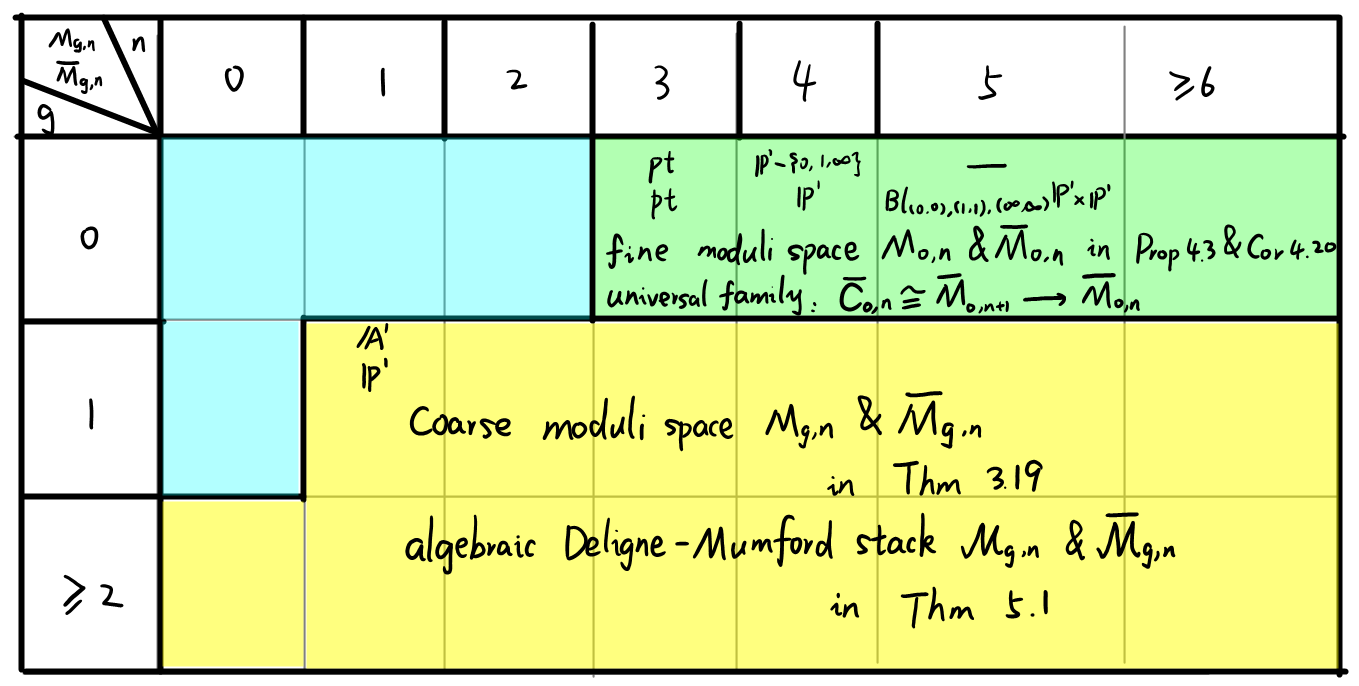
\includegraphics[width=12cm]{figures/moduliofcurve.png}
    \label{fig:moduliofcurve}
    \caption{The moduli of curves}
        
\end{figure} 
%%%%%%%%%%%%%%%%%%%%%%%%%%%%%%%%%%%%%%%%%%%%%%%%%%%%%%%%%%%%%%%%%%%%%%%%%%%%%%%%%%%%%%%%%%%%%
\section{Moduli of elliptic curve}
The elliptic curve theory is especially rich compared to the other curves. That's why we'd like to put it a special section.
\subsection{Definition and basic properties of elliptic curve}
\begin{defn}[Relative elliptic curve]
Let $S \in \Ob(\Schk)$. An $S$-group scheme $(E,m)$ is called an elliptic curve over $S$ if the structure map $\pi: E\longrightarrow S$ is proper, smooth of relative dimension $1$, and has connected fibers. Two elliptic curves are considered as the same if they are isomorphic as the $S$-group scheme.
\end{defn}
This data is equivalent to what we described for $\mathcal{M}_{1,1}(S)$ in Definition \ref{def:moduliofcurves}, and also equivalent to the definition in \cite[\href{https://stacks.math.columbia.edu/tag/072J}{Tag 072J}]{stacks-project}. 

Recall the Cohomology and Base Change Theorem in \cite[28.1.6]{FOAG}. Here we just give a simplified version:
\begin{theorem}[Cohomology and Base Change Theorem, simplified version]\label{thm:cohbc} $\hspace{0cm}$

	\begin{minipage}[t]{.6\textwidth}
	\vspace{-1cm}
Suppose		
\begin{itemize}
\item $S$ is locally Noetherian;
\item $\pi: X \longrightarrow S$ is proper;
\item The coherent sheaf $\mathcal{F}$ over $X$ is flat over $S$.
\end{itemize}
	\end{minipage}
\hfill\vline\hfill
	\begin{minipage}[b]{.36\textwidth}
		\centering
% https://q.uiver.app/?q=WzAsNSxbMCwxLCJYX3EiXSxbMSwxLCJYIl0sWzAsMiwiXFxTcGVjXFwsIFxca2FwcGEocSkiXSxbMSwyLCJTIl0sWzIsMCwiXFxtYXRoY2Fse0Z9Il0sWzAsMV0sWzAsMiwiXFxwaV9xIiwyXSxbMiwzLCJcXGlvdGEiXSxbMSwzLCJcXHBpIl0sWzQsMSwiIiwwLHsic3R5bGUiOnsiaGVhZCI6eyJuYW1lIjoibm9uZSJ9fX1dXQ==
\[\begin{tikzcd}
	&[-3mm]&[-5mm] {\mathcal{F}} \\[-6mm]
	{X_q} & X \\
	{\hspace{-0.8cm}\Spec\, \kappa(q)} & S
	\arrow[from=2-1, to=2-2]
	\arrow["{\pi_q}"', from=2-1, to=3-1]
	\arrow["\iota", from=3-1, to=3-2]
	\arrow["\pi", from=2-2, to=3-2]
	\arrow[no head, from=1-3, to=2-2]
\end{tikzcd}\]
	\end{minipage}
then for any $q \in S$ and $p \in \mathbb{Z}$, we have the  natural map
$$\phi^p_q: (\rderiv{p}{\pi_*}  \mathcal{F})|_q \longrightarrow H^p(X_q,\mathcal{F}|_{X_q})$$
which has the following properties:
$$\phi^p_q \text{ is surj } \Longrightarrow \begin{cases}
\hspace{2.6mm}\phi^p_q \text{ is iso }\\
\left(\phi^{p-1}_q \text{ is surj } \Leftrightarrow \rderiv{p}{\pi_*}  \mathcal{F} \text{ is l.f. }\right)
\end{cases}$$
\end{theorem}

We can use Theorem \ref{thm:cohbc} to compute some pushforward of sheaves, and the results are shown here:
\begin{table}[ht]
\[
\begin{array}{|r|c|c|c|c|c|c|c|}
\hline
n                                   & -3                    & -2                    & -1          & 0             & 1           & 2                     & 3                     \\ \hline
\rderiv{1}{\pi_*} \mathcal{O}_E(ne) & \text{rank 3} & \text{rank 2} & \text{l.b.} & \text{l.b.}   & 0           & 0                     & 0                     \\ \hline
\pi_* \mathcal{O}_E(ne)             & 0                     & 0                     & 0           & \mathcal{O}_S & \text{l.b.} & \text{rank 2} & \text{rank 3} \\ \hline
\rderiv{1}{\pi_*} \Omega_{E/S}(ne)  & \text{rank 3} & \text{rank 2} & \text{l.b.} & \mathcal{O}_S & 0           & 0                     & 0                     \\ \hline
\pi_* \Omega_{E/S}(ne)              & 0                     & 0                     & 0           & \text{l.b.}   & \text{l.b.} & \text{rank 2} & \text{rank 3} \\ \hline
\end{array}
\]
\end{table}
\begin{eg}[{case of $\rderiv{p}{\pi_*} \mathcal{O}_E$}]
Let $X=E$ be an elliptic curve over $S$, $\mathcal{F}=\mathcal{O}_X$. Obviously $\phi_q^2,\phi_q^{-1}$ are surjective; the map $\phi_q^{0}$ is also surjective\footnote{see the hint in \cite[28.1.H]{FOAG}.}. By using Theorem \ref{thm:cohbc} (see the Figure \ref{fig:cohbc1}) we obtain that $$\rderiv{p}{\pi_*} \mathcal{O}_X= \begin{cases}
0 & p \geqslant 2 \\
\text{line bundle} & p=0,1
\end{cases}$$
\end{eg}
\begin{figure}[ht]
\centering
\begin{tikzpicture}[node distance=5mm and 15mm, 
initial/.style={
color=red,
}]
\node (phiq2) [initial] {$\phi_q^2$ is surj};
\node (phiq1) [below right=of phiq2] {$\phi_q^1$ is surj};
\node (phiq0) [below right=of phiq1, initial] {$\phi_q^0$ is surj};
\node (phiq-1) [below right=of phiq0, initial] {$\phi_q^{-1}$ is surj};
\node (fiber2) [above right=of phiq2] {$\rderiv{2}{\pi_*}\mathcal{F}|_q=0$};
\node (fiber1) [above right=of phiq1] {$\rderiv{1}{\pi_*}\mathcal{F}|_q \cong \kappa(q)$};
\node (fiber0) [above right=of phiq0] {$\pi_*\mathcal{F}|_q\cong \kappa(q)$};
\node (lf2) [right=of phiq2] {$\rderiv{2}{\pi_*}\mathcal{F}$ is l.f.};
\node (lf1) [right=of phiq1] {$\rderiv{1}{\pi_*}\mathcal{F}$ is l.f.};
\node (lf0) [right=of phiq0] {${\pi_*}\mathcal{F}$ is l.f.};
\path ($ (lf2.south west) + (10mm,0) $) edge[commutative diagrams/Rightarrow, 2tail reversed] ($ (phiq1.north west) + (10mm,0) $);
\path ($ (lf1.south west) + (10mm,0) $) edge[commutative diagrams/Rightarrow, 2tail reversed] ($ (phiq0.north west) + (10mm,0) $);
\path ($ (lf0.south west) + (10mm,0) $) edge[commutative diagrams/Rightarrow, 2tail reversed] ($ (phiq-1.north west) + (10mm,0) $);
\path ($ (fiber2.south west) + (10mm,0) $) edge[->,edge label=Nakayama, red] ($ (lf2.north west) + (10mm,0) $);
\draw [->]
(phiq2.east)
-- ($ (phiq2.east) + (12mm,0) $)
|- (fiber2.west);
\draw [->]
($ (phiq2.east) + (12mm,0) $)
|- ($ (lf2.south west)!0.5!(phiq1.north west) + (8mm,0)$);
\draw [->]
(phiq1.east)
-- ($ (phiq1.east) + (12mm,0) $)
|- (fiber1.west);
\draw [->]
($ (phiq1.east) + (12mm,0) $)
|- ($ (lf1.south west)!0.5!(phiq0.north west) + (8mm,0)$);
\draw [->]
(phiq0.east)
-- ($ (phiq0.east) + (12mm,0) $)
|- (fiber0.west);
\draw [->]
($ (phiq0.east) + (12mm,0) $)
|- ($ (lf0.south west)!0.5!(phiq-1.north west) + (8mm,0)$);
\end{tikzpicture}
\caption{the process; \textcolor{red}{red} color is the initial condition}
\label{fig:cohbc1}
\end{figure}
\begin{lemma}
$\pi_*\mathcal{O}_X \cong \mathcal{O}_S$.
\end{lemma}
\begin{proof}
The morphism $\pi: X \longrightarrow S$ induces the map of sheaves
$$\pi^{\#}: \mathcal{O}_S \longrightarrow \pi_*\mathcal{O}_X$$
which corresponds a section of $\pi_*\mathcal{O}_X$. Since $\pi_*\mathcal{O}_X$ is a line bundle, this section defines a Cartier divisor $D$ of $S$, i.e. $\pi_*\mathcal{O}_X \cong \mathcal{O}_S(D)$. From the isomorphism 
$$\pi^{\#}|_q : \kappa(q) \longrightarrow \pi_*\mathcal{O}_X \times_{\mathcal{O}_S} \kappa(q) \textcolor{ashgrey}{ \stackrel{\phi_q^0}{\longrightarrow}H^0(X_q,\mathcal{O}_{X_q}) \cong \kappa(q) }$$
we get $D=0$, thus $\pi_*\mathcal{O}_X \cong \mathcal{O}_S$.
\end{proof}

\begin{remark}
The other cases are similarly solved except $\mathcal{F}=\Omega_{E/S}$. Actually, if we admit the Grothendieck-Serre duality
$$\rderiv{p}{\pi_*}\Omega_{E/S} \cong (\rderiv{1-p}{\pi_*} \mathcal{O}_E)^{\vee}$$
this would be easily solved. You can see the discussion \href{https://math.stackexchange.com/questions/1938206/local-freeness-of-the-hodge-bundle}{here} for Exercise \cite[28.1.N]{FOAG}, and \cite[2.1.2]{hida2011geometric} for the ``proof" of Grothendieck-Serre duality. For me the question in stackexchange is still unsolved, and for solving Exercise \cite[28.1.N]{FOAG} one need to assume the base scheme is reduced to use the Grauert’s Theorem in \cite[28.1.5]{FOAG}.(The Figure \ref{fig:cohbc2} shows where we use the Grauert’s Theorem.)
\end{remark}
\begin{table}[ht]
\begin{tabular}{@{}lll@{}}
\toprule
\multicolumn{1}{c}{Method} & \multicolumn{1}{c}{Result} & \multicolumn{1}{c}{Requirement} \\ \midrule
Grothendieck-Serre duality & $\rderiv{1}{\pi_*}\mathcal{F} \cong \mathcal{O}_E$ & haven't checked \\
Grauert's theorem & $\rderiv{1}{\pi_*}\mathcal{F}$ is l.f. & $S$ is reduced \\
$\Omega_{E/S} \cong \mathcal{O}_E$ locally & $\rderiv{1}{\pi_*}\mathcal{F}$ is l.f. & $E/S$ is group scheme \\ \bottomrule
\end{tabular}
\caption{}
\end{table}
\begin{figure}[ht]
\centering
\begin{tikzpicture}[node distance=5mm and 15mm, 
initial/.style={
color=red,
}]
\node (phiq2) [initial] {$\phi_q^2$ is surj};
\node (phiq1) [below right=of phiq2] {$\phi_q^1$ is surj};
\node (phiq0) [below right=of phiq1] {$\phi_q^0$ is surj};
\node (phiq-1) [below right=of phiq0, initial] {$\phi_q^{-1}$ is surj};
\node (fiber2) [above right=of phiq2] {$\rderiv{2}{\pi_*}\mathcal{F}|_q=0$};
\node (fiber1) [above right=of phiq1] {$\rderiv{1}{\pi_*}\mathcal{F}|_q \cong \kappa(q)$};
\node (fiber0) [above right=of phiq0] {$\pi_*\mathcal{F}|_q\cong \kappa(q)$};
\node (lf2) [right=of phiq2] {$\rderiv{2}{\pi_*}\mathcal{F}$ is l.f.};
\node (lf1) [right=of phiq1] {$\rderiv{1}{\pi_*}\mathcal{F}$ is l.f.};
\node (lf0) [right=of phiq0] {${\pi_*}\mathcal{F}$ is l.f.};
\path ($ (lf2.south west) + (10mm,0) $) edge[commutative diagrams/Rightarrow, 2tail reversed] ($ (phiq1.north west) + (10mm,0) $);
\path ($ (lf1.south west) + (10mm,0) $) edge[commutative diagrams/Rightarrow, 2tail reversed] ($ (phiq0.north west) + (10mm,0) $);
\path ($ (lf0.south west) + (10mm,0) $) edge[commutative diagrams/Rightarrow, 2tail reversed] ($ (phiq-1.north west) + (10mm,0) $);
\path ($ (fiber2.south west) + (10mm,0) $) edge[->,edge label=Nakayama, red] ($ (lf2.north west) + (10mm,0) $);
\path ($ (fiber1.south west) + (10mm,0) $) edge[->,edge label=Grauert, blue] ($ (lf1.north west) + (10mm,0) $);
\draw [->]
(phiq2.east)
-- ($ (phiq2.east) + (12mm,0) $)
|- (fiber2.west);
\draw [->]
($ (phiq2.east) + (12mm,0) $)
|- ($ (lf2.south west)!0.5!(phiq1.north west) + (8mm,0)$);
\draw [->]
(phiq1.east)
-- ($ (phiq1.east) + (12mm,0) $)
|- (fiber1.west);
\draw [->]
($ (phiq1.east) + (12mm,0) $)
|- ($ (lf1.south west)!0.5!(phiq0.north west) + (8mm,0)$);
\draw [->]
(phiq0.east)
-- ($ (phiq0.east) + (12mm,0) $)
|- (fiber0.west);
\draw [->]
($ (phiq0.east) + (12mm,0) $)
|- ($ (lf0.south west)!0.5!(phiq-1.north west) + (8mm,0)$);
\end{tikzpicture}
\caption{$\mathcal{F}=\Omega_{E/S}$; \textcolor{red}{red} color is the initial condition}
\label{fig:cohbc2}
\end{figure}
\begin{remark}
In the case that $X=E$ is an elliptic curve over $S$, we know more about the Hodge bundle $\pi_*\Omega_{E/S}$ than just a line bundle:
\begin{itemize}
\item $(\pi_*\Omega_{E/S})^{E}=\pi_*\Omega_{E/S}$ since any global differential on an Abelian variety is invarient; % Comes from https://mathoverflow.net/questions/334428/definition-of-an-invariant-differential-of-an-elliptic-curve
\item By \cite[Proposition 3.15]{saito2014fermat}, the line bundle $\omega_{E/S}:=e^*\Omega_{E/S}$ is isomorphic to the Hodge bundle $\pi_*\Omega_{E/S}$. As a corollary, we get
$$\Omega_{E/S} \stackrel{\text{gp sch}}{\cong} \pi^* e^* \Omega_{E/S} = \pi^* \omega_{E/S} \cong \pi^* \pi_* \Omega_{E/S}.$$
\end{itemize}
\end{remark}
\subsection{Differential}
We know that $\mathcal{M}_{1,1}$ is not representable, so we have to introduce extra structures to rigidify elliptic curves. The first possible extra structure is the differential.
\begin{defn}[{Weierstrass moduli $\widetilde{\mathcal{M}}\!\left[\textstyle \frac{1}{6}\right]$}]
For a base scheme $S \in \Ob(\Sch_{\mathbb{Z}\left[\frac{1}{6} \right]})$, we define a moduli problem
$$\mathcal{A}_S:=\left\{(E,\omega)  \;\middle|\; \begin{aligned}
&\\[-5mm]
& E: \text{ elliptic curve over } S \\[-1mm]
& \omega \in \Gamma(E,\Omega_{E/S}) \text{ global generator }
\end{aligned}
 \right\}$$
 
   $(E,\omega) \sim_S (E',\omega')$ if there exists an isomorphism of elliptic curves $\phi:E \longrightarrow E'$ such that $\omega'=\phi^* \circ \omega'$.
   
   For a map $f:T \longrightarrow S$, the pullback $f^*$ is defined by
      $$f^*:\mathcal{A}_S \longrightarrow \mathcal{A}_T \qquad (E,\omega) \longmapsto \big(f^*E,f^*  \omega\big)$$
      
      By doing so we define the moduli functor 
      $$\widetilde{\mathcal{M}}\!\left[\textstyle \frac{1}{6}\right]: \Sch_{\mathbb{Z}\left[\frac{1}{6} \right]} \longrightarrow \Set \qquad S \longmapsto \mathcal{A}_S/\sim_S$$
\end{defn}
\begin{theorem}
The moduli functor $\widetilde{\mathcal{M}}\!\left[\textstyle \frac{1}{6}\right]$ is represented by $\Spec \mathbb{Z}\!\left[\textstyle \frac{1}{6}\right] \left[a,b, \Delta^{-1} \right]$ where $\Delta=-\frac{1}{256}(4a^3+27b^2)$. Denote $R=\mathbb{Z}\!\left[\textstyle \frac{1}{6}\right] \left[a,b, \Delta^{-1} \right]$, the universal family is $(E_R,\omega_R) \in \widetilde{\mathcal{M}}\!\left[\textstyle \frac{1}{6}\right](R)$, where
\begin{equation*}
\begin{aligned}
  E_R=\;& \Proj R[x,y,z]/\left( y^2z-(x^3+axz^2+bz^3) \right)  \\ 
  \omega_R=\;&  \frac{x\dd z-z\dd x}{2yz}=\frac{y\dd z-z\dd y }{3x^2+az^2} =\frac{x\dd y-y\dd x}{y^2-2axz-3bz^2} \quad\text{ whenever it's defined.}\\ 
\end{aligned}
\end{equation*}
\end{theorem}
\begin{proof}
need complement. The idea is, consider it locally, find appropriate $1,x,y$ with respect to the differential $\omega$, and finally glue them.
\end{proof}
To be compatible with the notations in modular form, we rewrite
\begin{equation*}
\begin{aligned}
  R=\;&\mathbb{Z}\!\left[\textstyle \frac{1}{6}\right] \left[a,b, \Delta^{-1} \right] \cong \mathbb{Z}\!\left[\textstyle \frac{1}{6}\right] \left[g_2,g_3, \Delta^{-1} \right]  && a=-4g_2, b=-16g_3, \Delta=g_3^2-27g_3^2\\
  E_R=\;& \Proj R[x,y,z]/\left( y^2z-(4x^3-g_2xz^2-g_3z^3) \right) && \text{\textcolor{ashgrey}{here $x$ is different}}\\ 
  \omega_R=\;&  \frac{x\dd z-z\dd x}{2yz}=\frac{y\dd z-z\dd y }{12x^2-g_2z^2} =\frac{x\dd y-y\dd x}{y^2+2g_2xz+3g_3z^2} &&\text{whenever it's defined.}\\ 
\end{aligned}
\end{equation*}

As an application, we prove that the coarse moduli of functor  $\mathcal{M}\!\left[ \frac{1}{6}\right]:=\mathcal{M}_{1,1}\!\left[ \frac{1}{6}\right]$ is $\mathbb{A}^1_{\mathbb{Z} \!\left[ \frac{1}{6}\right]}$. Recall that $\mathbb{G}_m$ acts on $\widetilde{\mathcal{M}}\!\left[\textstyle \frac{1}{6}\right]$ by
$$R \longrightarrow R \times_{\mathbb{Z}} \mathbb{Z}[t,t^{-1}] \cong R[t,t^{-1}] \qquad g_2\longmapsto t^{-4}g_2 \quad g_3 \longrightarrow t^{-6}g_3,$$
thus $\mathbb{G}_m(S)$ acts on $\widetilde{\mathcal{M}}\!\left[\textstyle \frac{1}{6}\right](S)$ by
$$\mathbb{G}_m(S) \times \widetilde{\mathcal{M}}\!\left[\textstyle \frac{1}{6}\right](S) \longrightarrow \widetilde{\mathcal{M}}\!\left[\textstyle \frac{1}{6}\right](S) \qquad \big(u, (E,\omega) \big) \longmapsto \big(E, u^{\#}(t) \cdot \omega \big).$$
Define
$$j:=1728\frac{g_2^3}{\Delta}=1728\frac{g_2^3}{g_3^2-27g_3^2}\in R^{\mathbb{G}_m},$$
by tedious check we get
$$R^{\mathbb{G}_m} = \mathbb{Z} \!\left[ \textstyle\frac{1}{6}\right][j]$$
which induce the isomorphism 
$$j: \mathbb{G}_m\backslash \widetilde{\mathcal{M}}\!\left[\textstyle \frac{1}{6}\right] \longrightarrow \mathbb{A}^1_{\mathbb{Z} \!\left[ \frac{1}{6}\right]}.$$
\begin{claim}
The scheme $\mathbb{G}_m\backslash \widetilde{\mathcal{M}}\!\left[\textstyle \frac{1}{6}\right] \cong \mathbb{A}^1_{\mathbb{Z} \!\left[ \frac{1}{6}\right]}$ is the course moduli of $\mathcal{M}\!\left[ \frac{1}{6}\right]$.
\begin{figure}[ht]
\centering
% https://q.uiver.app/?q=WzAsNCxbMCwxLCJcXG1hdGhjYWx7TX1cXCFcXGxlZnRbIFxcZnJhY3sxfXs2fVxccmlnaHRdIl0sWzIsMSwiXFxtYXRoYmJ7R31fbVxcYmFja3NsYXNoIFxcd2lkZXRpbGRle1xcbWF0aGNhbHtNfX1cXCFcXGxlZnRbXFx0ZXh0c3R5bGUgXFxmcmFjezF9ezZ9XFxyaWdodF0iXSxbMiwyLCJoX3tYJ30iXSxbMSwwLCJcXHdpZGV0aWxkZXtcXG1hdGhjYWx7TX19XFwhXFxsZWZ0W1xcdGV4dHN0eWxlIFxcZnJhY3sxfXs2fVxccmlnaHRdIl0sWzAsMSwiXFxldGEiXSxbMSwyLCJcXGV4aXN0cyBcXCwhIFxcLGhfe1xcYmV0YX0iLDAseyJjb2xvdXIiOlszNTgsMTAwLDUwXSwic3R5bGUiOnsiYm9keSI6eyJuYW1lIjoiZGFzaGVkIn19fSxbMzU4LDEwMCw1MCwxXV0sWzAsMiwiXFxhbHBoYSciLDJdLFszLDAsIlxcdGV4dHtmb3JnZXR9IiwyLHsibGFiZWxfcG9zaXRpb24iOjYwfV0sWzMsMSwiXFx0ZXh0e3F1b3RpZW50fSIsMCx7ImxhYmVsX3Bvc2l0aW9uIjo2MH1dXQ==
\[\begin{tikzcd}
	& {\widetilde{\mathcal{M}}\!\left[\textstyle \frac{1}{6}\right] \makebox[0pt][l]{\textcolor{ashgrey}{$\cong h_{\Spec R}$}}} \\
	{\mathcal{M}\!\left[ \frac{1}{6}\right]} && {\mathbb{G}_m\backslash \widetilde{\mathcal{M}}\!\left[\textstyle \frac{1}{6}\right]\makebox[0pt][l]{\textcolor{ashgrey}{$\cong h_{\mathbb{A}^1_{\mathbb{Z}\left[ 1/6\right]}}$}}} \\
	&& {h_{X'}}
	\arrow["\eta", from=2-1, to=2-3]
	\arrow["{\exists \,! \,h_{\beta}}", color={rgb,255:red,255;green,0;blue,8}, dashed, from=2-3, to=3-3]
	\arrow["{\alpha'}"', from=2-1, to=3-3]
	\arrow["{\text{forget}}"'{pos=0.6}, from=1-2, to=2-1]
	\arrow["{\text{quotient}}"{pos=0.6}, from=1-2, to=2-3]
\end{tikzcd}\]
\caption{verification of coarse moduli}
\label{fig:coarsemoduliofell}
\end{figure}
\end{claim}
\begin{proof}
We check it by the definition of coarse moduli, see Figure \ref{fig:coarsemoduliofell}.
\subsectiondisappear*{\underline{Step1}}
Construct $\eta$. To define \textcolor{ashgrey}{($S \in \Sch_{\mathbb{Z}\left[\frac{1}{6} \right]}$)}
$$\eta(S): \mathcal{M}\!\left[\textstyle \frac{1}{6}\right](S) \longrightarrow \mathbb{G}_m\backslash \widetilde{\mathcal{M}}\!\left[\textstyle \frac{1}{6}\right](S) \cong \Gamma(S,\mathcal{O}_S),$$
we first find differential locally (locally lift to $\widetilde{\mathcal{M}}\!\left[\textstyle \frac{1}{6}\right]$)\footnote{We know that $\Omega_{E/S} \cong \pi^*e^*\Omega_{E/S} \stackrel{loc}{\cong} \pi^*\mathcal{O}_S \cong \mathcal{O}_X$ locally.}, and then take quotient. You need to check:
\begin{itemize}
\item $j$-function doesn't depend on the choice of differential, so $\eta(S)$ is well-defined;
\item $\eta$ is really a functor.
\end{itemize}
\subsectiondisappear*{\underline{Step2}}
We know that GIT quotient is a categorical quotient, so there exists unique $h_{\beta}$ such that 
$$h_{\beta} \circ \text{quotient} = \alpha' \circ \text{forget}.$$
You need to check $\alpha'=h_{\beta} \circ \eta$.
\end{proof}
\subsectiondisappear*{\underline{Step3}}
For any closed field $k=\bar{k}$, $\chara k\neq 2,3$, the map
$$\eta(k): \mathcal{M}\!\left[\textstyle \frac{1}{6}\right](k) \longrightarrow \mathbb{G}_m\backslash \widetilde{\mathcal{M}}\!\left[\textstyle \frac{1}{6}\right](k) \cong k$$
is an isomorphism.
\subsection{Crash course on Abelian variety}
When I was reading some materials about the level structure of elliptic curve, I realised that I'm still not so familiar with some fine structure of elliptic curve, such as $E[n]$. It's usually done as the special case of the Abelian variety\footnote{There are thousands of books talking about elliptic curves, but most of them are unrelavent to us: some restrict themselves to the complex field $\mathbb{C}$, some focus on the applications of cryptography, and some prove every result by the Weierestrass equation, in a very down to earth but ugly way. }. The standard reference is \cite{mumford1974abelian,milne1986abelian}, but we would follow instead \cite{edixhoven2012abelian}\footnote{Be careful that there are a lot of versions in the internet, and the latest verion (as far as I know) is \href{http://van-der-geer.nl/~gerard/AV.pdf}{here}. Unless otherwise specified we cite for the main part of the text rather than the exercises.} since it's much less disgusting to read.

As a lazy guy, I would instead list main tasks in \cite{edixhoven2012abelian}:
\begin{itemize}
\item State the theorem of cubic, and show that 
$$[n]^*\mathcal{L} \cong \mathcal{L}^{\otimes \frac{n(n+1)}{2}} \otimes ([-1]^* \mathcal{L})^{\otimes \frac{n(n-1)}{2}}$$
\item Understand torsion points $X[n]$.
\begin{itemize}
\item Define isogeny(5.3) and isogenous(5.13);
\item Give the canonical factorization of an isogeny(5.8)\footnote{Analog: any field extension can be uniquely written as an inseparable extension with a separable extension.};
\item Examples of isogeny: $[n], F, V$\footnote{$[n]$ is an isogeny when $n \neq 0$; $F$ and $V$ are defined when $\chara k=p>0$.}. Find their relationships(5.19, 5.20);
\item Describe the kernel of isogeny: $X[n], X[F], X[V]$(5.11, 5.22, not completed). 

In char $p$ case, define the relevant notions: $p$-rank, ordinary, supersingular(5.23, 5.25). 

When $p=2,3$, describe the criterian for an elliptic curve to be supersingular(5.26, 5.27). 

When $p=2$, describe the action $\alpha_2$ on $X \subseteq \mathbb{P}_k^2: y^2z+yz^2=x^3$, and show that $X[F] \cong \alpha_2$(5.28). 

For more informations about supersingular curve, see \href{https://en.wikipedia.org/wiki/Supersingular_elliptic_curve}{wiki} and \cite[Proposition 8.2]{saito2014fermat}. 
\end{itemize}
\item Understand Picard group, dual, Weil pairing and Tate modules. I haven't read about it.
\end{itemize} 
\subsection{Level structure}
The second possible extra structure is the level structure.
\subsection{Complex case}
In this subsection, we will show that how the moduli is connected to the modular curve $\mathcal{H}/\SL_2(\mathbb{Z})$.

%%%%%%%%%%%%%%%%%%%%%%%%%%%%%%%%%%%%%%%%%%%%%%%%%%%%%%%%%%%%%%%%%%%%%%%%%%%%%%%%%%%%%%%%%%%%%
\section{Moduli of higher dimensional variety, MMP}
I would add something here if I know.
\subsection{Moduli of algebraic surfaces}
We know the Enriques–Kodaira classification, which contributes to a better understanding of algebraic surfaces. But that's not enough. Do we know the classification of K3-surfaces?
\subsection{MMP}
Here we refer to the survey \cite{xu2020kstability}, or the \href{https://math.mit.edu/~cyxu/Kstability.pdf}{updated version}. You can get a glimpse of the current progress in MMP (especially in the table of page 63).
%%%%%%%%%%%%%%%%%%%%%%%%%%%%%%%%%%%%%%%%%%%%%%%%%%%%%%%%%%%%%%%%%%%%%%%%%%%%%%%%%%%%%%%%%%%%%
\section{Moduli of vector bundle}
The course lecture note \href{https://userpage.fu-berlin.de/hoskins/moduli_and_GIT.html}{``Moduli and GIT"} would be a perfect survey to begin with. We also refer to \cite{huybrechts2010geometry}. It's not easy to read, but It's in some sense completed, and everybody refers it.

For a variant, you may get some informations of moduli of $G$-bundles over elliptic curve in \cite{frăţilă2020revisiting}.
\bibliographystyle{plain}
\bibliography{reference}





\end{document}

%流程图模板
%\usetikzlibrary {positioning,shapes.misc}
%\begin{tikzpicture}[node distance=5mm and 10mm, 
%initial/.style={
%color=red,
%}]
%\node (phiq2) [initial] {$\phi_q^2$ is surj};
%\node (phiq1) [below right=of phiq2] {$\phi_q^1$ is surj};
%\node (phiq0) [below right=of phiq1] {$\phi_q^0$ is surj};
%\node (phiq-1) [below right=of phiq0] {$\phi_q^{-1}$ is surj};
%\node (fiber2) [above right=of phiq2] {$\rderiv{2}{\pi_*}\mathcal{F}|_q$};
%\node (fiber1) [above right=of phiq1] {$\rderiv{1}{\pi_*}\mathcal{F}|_q$};
%\node (fiber0) [above right=of phiq0] {$\pi_*\mathcal{F}|_q$};
%\node (lf2) [right=of phiq2] {$\rderiv{2}{\pi_*}\mathcal{F}$ is l.f.};
%\node (lf1) [right=of phiq1] {$\rderiv{1}{\pi_*}\mathcal{F}$ is l.f.};
%\node (lf0) [right=of phiq0] {${\pi_*}\mathcal{F}$ is l.f.};
%\path ($ (lf2.south west) + (10mm,0) $) edge[commutative diagrams/Rightarrow, 2tail reversed] ($ (phiq1.north west) + (10mm,0) $);
%\path ($ (lf1.south west) + (10mm,0) $) edge[commutative diagrams/Rightarrow, 2tail reversed] ($ (phiq0.north west) + (10mm,0) $);
%\path ($ (lf0.south west) + (10mm,0) $) edge[commutative diagrams/Rightarrow, 2tail reversed] ($ (phiq-1.north west) + (10mm,0) $);
%\draw [->]
%(phiq2.east)
%-- ($ (phiq2.east) + (8mm,0) $)
%|- (fiber2.west);
%\draw [->]
%($ (phiq2.east) + (8mm,0) $)
%|- ($ (lf2.south west)!0.5!(phiq1.north west) + (8mm,0)$);
%\draw [->]
%(phiq1.east)
%-- ($ (phiq1.east) + (8mm,0) $)
%|- (fiber1.west);
%\draw [->]
%($ (phiq1.east) + (8mm,0) $)
%|- ($ (lf1.south west)!0.5!(phiq0.north west) + (8mm,0)$);
%\draw [->]
%(phiq0.east)
%-- ($ (phiq0.east) + (8mm,0) $)
%|- (fiber0.west);
%\draw [->]
%($ (phiq0.east) + (8mm,0) $)
%|- ($ (lf0.south west)!0.5!(phiq-1.north west) + (8mm,0)$);
%\end{tikzpicture}


